\documentclass{article}
\usepackage{graphicx}

\title{Práctica 0: Repaso de Java e introducci´on a Maven \\ Cómputo Concurrente 2024-2}
\author{Pérez Romero Natalia Abigail}
\date{\today}

\begin{document}
\maketitle

\section{Diagrama UML}

\begin{figure}[h]
    \centering
    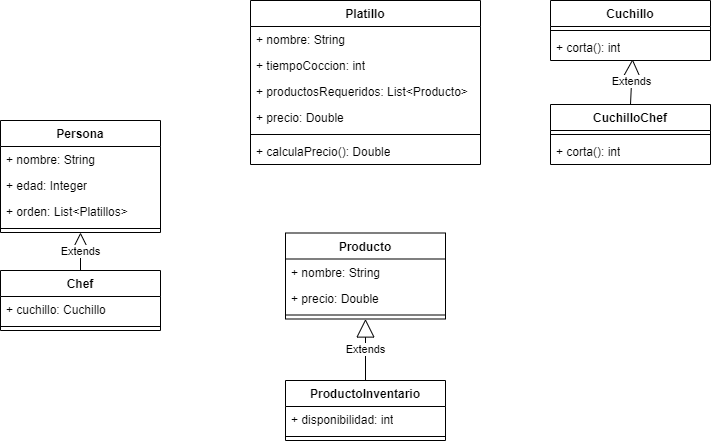
\includegraphics[width=\textwidth]{UML.png}
    \caption{Diagrama UML}
    \label{fig:UML}
\end{figure}

\section{Justificación de Patrones de Diseño}

Utilizo el patrón de diseño Strategy, en la clase Persona para permitir almacenar el pedido de una persona, de manera dinámica, es decir, que se pueda cambiar en tiempo de ejecución el algoritmo. Si se ordena un solo platillo, un producto o varios platillos no seria necesario cambiar la clase, solo se cambia el algoritmo que se va a utilizar.
 
También en esta clase utilizo el patrón de diseño Adapter, para poder atender el pedido de un solo producto.

\begin{figure}[h]
    \centering
    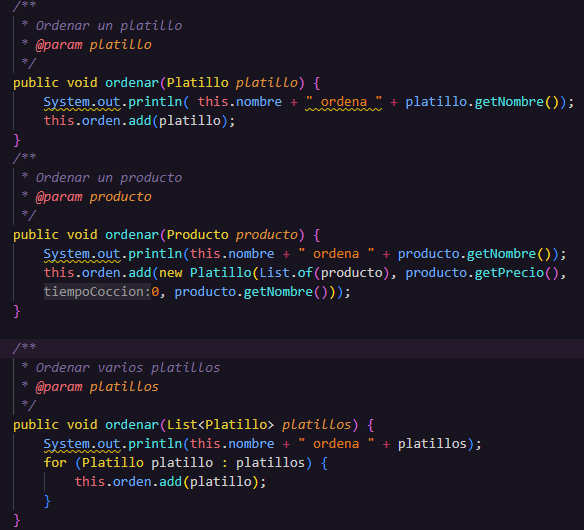
\includegraphics[width=\textwidth]{codigoPersona.png}
    \caption{Diagrama UML}
    \label{fig:UML}
\end{figure}

Luego en las clases Cuchillo-CuchilloChef, Persona-Chef, Producto-ProductoInventario podemos ver el patrón de diseño Decorator, ya que se pueden agregar atributos y métodos a las clases que implentan la interfaz Cuchillo o heredan de la clase Producto, Persona, que les permiten realizar otras operaciones como Chef que es capaz de cortar un producto o Persona que puede hacer un pedido.
\end{document}
